% Frame 1 : Initialisation et Log(Odds)
\begin{frame}{XGBoost (Classification) : Initialisation et Log(Odds)}
    \begin{columns}[T]
        \begin{column}{0.4\textwidth}
            \textbf{Jeu de données :}
            \vspace{0.1cm}
            
            \begin{table}
                \centering
                \scriptsize
                \begin{tabular}{|c|c|c|}
                    \hline
                    \textbf{Dosage} & \textbf{Couleur} & \textbf{Efficacité ($y$)} \\
                    \hline
                    2 & Rouge & 0 (Non) \\
                    8 & Vert & 1 (Oui) \\
                    12 & Vert & 1 (Oui) \\
                    18 & Rouge & 0 (Non) \\
                    \hline
                \end{tabular}
            \end{table}
            
            \begin{block}{Prédiction initiale $p_0$}
                \scriptsize
                Par défaut, on prédit $p_0 = \textbf{0.5}$ pour tout le monde.
                
                \vspace{0.1cm}
                Cependant, XGBoost construit ses arbres avec des \textbf{Log(Odds)} (Log-cotes).
                $$ \text{Log(Odds)} = \log\left(\frac{p}{1-p}\right) $$
                Si $p=0.5$, l'initialisation vaut $0$.
            \end{block}
        \end{column}
        
        \begin{column}{0.6\textwidth}
            \begin{center}
            \textbf{\footnotesize Résidus initiaux ($r_i = y_i - p_0$)}
            
            \vspace{0.2cm}
            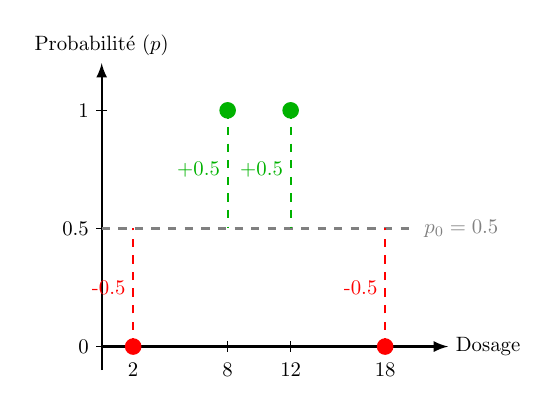
\begin{tikzpicture}[x=0.20cm, y=3cm, every node/.style={scale=0.75}]
                \draw[->, thick, -latex] (0,-0.1) -- (0,1.2) node[above] {Probabilité ($p$)};
                \draw[->, thick, -latex] (0,0) -- (22,0) node[right] {Dosage};
                
                \foreach \y in {0, 0.5, 1} { \draw (2pt,\y) -- (-2pt,\y) node[left] {\y}; }
                \foreach \x in {2, 8, 12, 18} { \draw (\x, 2pt) -- (\x, -2pt) node[below=2pt] {\x}; }
                
                \fill[red] (2,0) circle (3pt);
                \fill[green!70!black] (8,1) circle (3pt);
                \fill[green!70!black] (12,1) circle (3pt);
                \fill[red] (18,0) circle (3pt);
                
                \draw[thick, gray, dashed] (0, 0.5) -- (20, 0.5) node[right] {$p_0 = 0.5$};
                
                \draw[dashed, red, thick] (2,0) -- (2,0.5) node[midway, left] {-0.5};
                \draw[dashed, green!70!black, thick] (8,1) -- (8,0.5) node[midway, left] {+0.5};
                \draw[dashed, green!70!black, thick] (12,1) -- (12,0.5) node[midway, left] {+0.5};
                \draw[dashed, red, thick] (18,0) -- (18,0.5) node[midway, left] {-0.5};
            \end{tikzpicture}
            
            \vspace{0.2cm}
            \scriptsize
            Les pointillés montrent nos erreurs initiales ($r_i$). \\ XGBoost va s'en servir pour construire les arbres !
            \end{center}
        \end{column}
    \end{columns}
\end{frame}

% Frame 2 : Score de Similarite et Cover
\begin{frame}{XGBoost (Classification) : Score de Similarité}
    \begin{columns}[T]
        \begin{column}{0.5\textwidth}
            \begin{block}{Nouveau Score de Similarité ($SS$)}
                \small
                La formule s'adapte pour lier les probabilités (les résidus) et l'espace Log(Odds) des feuilles :
                $$ SS = \frac{(\sum \text{Résidus}_i)^2}{\sum \text{Cover}_i + \lambda} $$
            \end{block}
            
            \begin{block}{Calcul de la Racine ($\lambda=0$)}
                \scriptsize
                Pour le nœud racine (les 4 patients) :
                \begin{itemize}
                    \setlength\itemsep{0em}
                    \item $\sum r_i = (-0.5) + 0.5 + 0.5 - 0.5 = 0$
                    \item Numérateur : $0^2 = \textbf{0}$.
                \end{itemize}
                
                $$ \text{Score Racine} = \frac{0}{1.0 + 0} = \textbf{0} $$
            \end{block}
        \end{column}
        
        \begin{column}{0.5\textwidth}
            \begin{block}{La notion de "Cover" (Couverture)}
                \small
                Remplace le nombre d'observations ($N$) par la \textbf{variance} des prédictions précédentes :
                $$ \text{Cover}_i = p_i \times (1 - p_i) $$
                
                \footnotesize
                \vspace{0.1cm}
                Ici, comme $p_0=0.5$ pour tous :
                $$ \text{Cover}_i = 0.5 \times 0.5 = \textbf{0.25} $$
                
                \vspace{0.1cm}
                \textit{Le dénominateur total vaut donc :}
                $$ \sum \text{Cover}_i = 0.25 \times 4 = \textbf{1.0} $$
            \end{block}
        \end{column}
    \end{columns}
\end{frame}

% Frame 3 : Evaluation du Split A
\begin{frame}{XGBoost : Évaluation des Splits (Coupure à 5)}

    \begin{block}{Rappel : Gain}
        \scriptsize $ \text{Gain} = SS_{gauche} + SS_{droit} - SS_{racine} - \gamma $. Testons notre premier split !
    \end{block}

    \begin{columns}[T]
        \begin{column}{0.4\textwidth}
            \begin{block}{\textbf{Split A : Dosage < 5}}
                \scriptsize
                \textbf{Gauche (Dosage 2)} :
                \begin{itemize}
                    \setlength\itemsep{0em}
                    \item $\sum r = -0.5$
                    \item $SS_{G} = \frac{(-0.5)^2}{0.25} = \textbf{1.0}$
                \end{itemize}
                
                \textbf{Droit (Dosages 8, 12, 18)} :
                \begin{itemize}
                    \setlength\itemsep{0em}
                    \item $\sum r = 0.5 + 0.5 - 0.5 = 0.5$
                    \item $SS_{D} = \frac{(0.5)^2}{0.25 \times 3} = \textbf{0.33}$
                \end{itemize}
                
                $$ \text{Gain} = 1.0 + 0.33 - 0 = \textbf{1.33} $$
            \end{block}
        \end{column}
        
        \begin{column}{0.6\textwidth}
            \begin{center}
            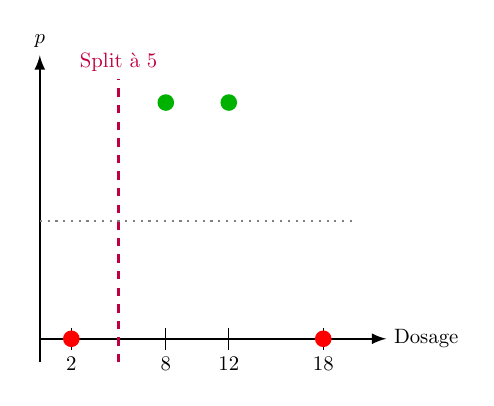
\begin{tikzpicture}[x=0.20cm, y=3cm, every node/.style={scale=0.75}]
                \draw[->, thick, -latex] (0,-0.1) -- (0,1.2) node[above] {$p$};
                \draw[->, thick, -latex] (0,0) -- (22,0) node[right] {Dosage};
                
                \foreach \x in {2, 8, 12, 18} { \draw (\x, 4pt) -- (\x, -4pt) node[below] {\x}; }
                
                \fill[red] (2,0) circle (3pt);
                \fill[green!70!black] (8,1) circle (3pt);
                \fill[green!70!black] (12,1) circle (3pt);
                \fill[red] (18,0) circle (3pt);
                
                % Ligne de split
                \draw[thick, purple, dashed] (5, -0.1) -- (5, 1.1) node[above] {Split à 5};
                
                \draw[thick, gray, dotted] (0, 0.5) -- (20, 0.5);
            \end{tikzpicture}
            
            \vspace{0.2cm}
            \scriptsize \textit{Isole la première valeur rouge. C'est un bon début !}
            \end{center}
        \end{column}
    \end{columns}
\end{frame}

% Frame 4 : Evaluation du Split B
\begin{frame}{XGBoost : Évaluation des Splits (Coupure à 10)}
    \begin{columns}[T]
        \begin{column}{0.4\textwidth}
            \begin{block}{\textbf{Split B : Dosage < 10}}
                \scriptsize
                \textbf{Gauche (Dosages 2, 8)} :
                \begin{itemize}
                    \setlength\itemsep{0em}
                    \item $\sum r = -0.5 + 0.5 = 0$
                    \item $SS_{G} = \frac{0^2}{0.5} = \textbf{0}$
                \end{itemize}
                
                \textbf{Droit (Dosages 12, 18)} :
                \begin{itemize}
                    \setlength\itemsep{0em}
                    \item $\sum r = 0.5 - 0.5 = 0$
                    \item $SS_{D} = \frac{0^2}{0.5} = \textbf{0}$
                \end{itemize}
                
                $$ \text{Gain} = 0 + 0 - 0 = \textbf{0} $$
            \end{block}
        \end{column}
        
        \begin{column}{0.6\textwidth}
            \begin{center}
            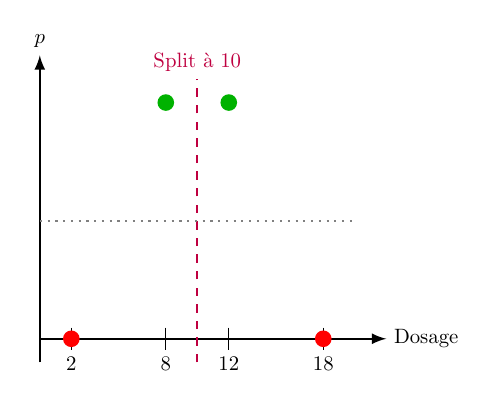
\begin{tikzpicture}[x=0.20cm, y=3cm, every node/.style={scale=0.75}]
                \draw[->, thick, -latex] (0,-0.1) -- (0,1.2) node[above] {$p$};
                \draw[->, thick, -latex] (0,0) -- (22,0) node[right] {Dosage};
                
                \foreach \x in {2, 8, 12, 18} { \draw (\x, 4pt) -- (\x, -4pt) node[below] {\x}; }
                
                \fill[red] (2,0) circle (3pt);
                \fill[green!70!black] (8,1) circle (3pt);
                \fill[green!70!black] (12,1) circle (3pt);
                \fill[red] (18,0) circle (3pt);
                
                % Ligne de split
                \draw[thick, purple, dashed] (10, -0.1) -- (10, 1.1) node[above] {Split à 10};
                
                \draw[thick, gray, dotted] (0, 0.5) -- (20, 0.5);
            \end{tikzpicture}
            
            \vspace{0.2cm}
            \scriptsize \textit{Mélange un rouge et un vert de chaque côté. \textbf{Pire split possible !}}
            \end{center}
        \end{column}
    \end{columns}
\end{frame}

% Frame 5 : Evaluation du Split C
\begin{frame}{XGBoost : Évaluation des Splits (Coupure à 15)}
    \begin{columns}[T]
        \begin{column}{0.4\textwidth}
            \begin{block}{\textbf{Split C : Dosage < 15}}
                \scriptsize
                \textbf{Gauche (Dosages 2, 8, 12)} :
                \begin{itemize}
                    \setlength\itemsep{0em}
                    \item $\sum r = -0.5 + 0.5 + 0.5 = 0.5$
                    \item $SS_{G} = \frac{0.5^2}{0.75} = \textbf{0.33}$
                \end{itemize}
                
                \textbf{Droit (Dosage 18)} :
                \begin{itemize}
                    \setlength\itemsep{0em}
                    \item $\sum r = -0.5$
                    \item $SS_{D} = \frac{(-0.5)^2}{0.25} = \textbf{1.0}$
                \end{itemize}
                
                $$ \text{Gain} = 0.33 + 1.0 - 0 = \textbf{1.33} $$
            \end{block}
        \end{column}
        
        \begin{column}{0.6\textwidth}
            \begin{center}
            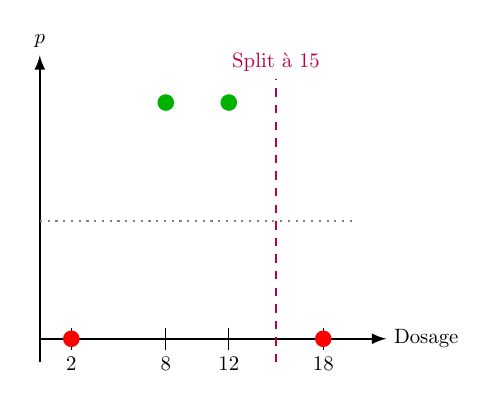
\begin{tikzpicture}[x=0.20cm, y=3cm, every node/.style={scale=0.75}]
                \draw[->, thick, -latex] (0,-0.1) -- (0,1.2) node[above] {$p$};
                \draw[->, thick, -latex] (0,0) -- (22,0) node[right] {Dosage};
                
                \foreach \x in {2, 8, 12, 18} { \draw (\x, 4pt) -- (\x, -4pt) node[below] {\x}; }
                
                \fill[red] (2,0) circle (3pt);
                \fill[green!70!black] (8,1) circle (3pt);
                \fill[green!70!black] (12,1) circle (3pt);
                \fill[red] (18,0) circle (3pt);
                
                % Ligne de split
                \draw[thick, purple, dashed] (15, -0.1) -- (15, 1.1) node[above] {Split à 15};
                
                \draw[thick, gray, dotted] (0, 0.5) -- (20, 0.5);
            \end{tikzpicture}
            
            \vspace{0.2cm}
            \scriptsize \textit{Gain = 1.33. Ex aequo avec le Split A ! Pourquoi le choisir ?} \\
            Parce qu'il sépare la classe majoritairement positive (Gauche) de la donnée la plus extrême (Celle de droite).
            \end{center}
        \end{column}
    \end{columns}
\end{frame}

% Frame 6 : Poursuite de la construction
\begin{frame}{XGBoost : Construction de l'Arbre 1 (Profondeur 2)}
    \vspace{-0.2cm}
    \begin{block}{Poursuite sur le Nœud Gauche (Dosages 2, 8, 12)}
        \scriptsize
        On teste à nouveau une coupure. Testons \textbf{Split D : Dosage < 5} sur ce sous-groupe :
    \end{block}
    
    \begin{columns}[T]
        \begin{column}{0.4\textwidth}
            \begin{block}{Évaluation du Split D}
                \scriptsize
                \textbf{Gauche (Dosage 2)} :
                \begin{itemize}
                    \setlength\itemsep{0em}
                    \item $\sum r = -0.5$
                    \item $SS_{G} = \frac{(-0.5)^2}{0.25} = \textbf{1.0}$
                \end{itemize}
                
                \textbf{Droit (Dosages 8, 12)} :
                \begin{itemize}
                    \setlength\itemsep{0em}
                    \item $\sum r = 0.5 + 0.5 = 1.0$
                    \item $SS_{D} = \frac{(1.0)^2}{0.5} = \textbf{2.0}$
                \end{itemize}
                
                Rappel $SS_{Racine Gauche} = \textbf{0.33}$
                $$ \text{Gain}_D = 1.0 + 2.0 - 0.33 = \textbf{2.67} $$
            \end{block}
        \end{column}
        
        \begin{column}{0.6\textwidth}
            \begin{center}
            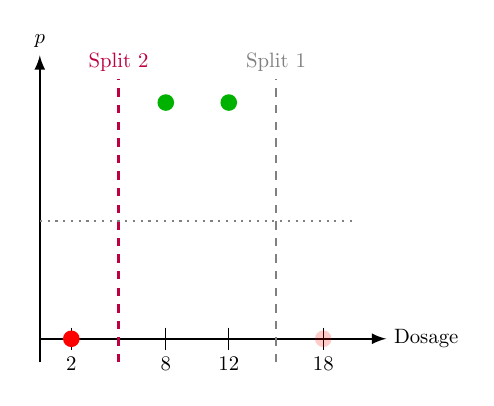
\begin{tikzpicture}[x=0.20cm, y=3cm, every node/.style={scale=0.75}]
                \draw[->, thick, -latex] (0,-0.1) -- (0,1.2) node[above] {$p$};
                \draw[->, thick, -latex] (0,0) -- (22,0) node[right] {Dosage};
                
                \foreach \x in {2, 8, 12, 18} { \draw (\x, 4pt) -- (\x, -4pt) node[below] {\x}; }
                
                \fill[red] (2,0) circle (3pt);
                \fill[green!70!black] (8,1) circle (3pt);
                \fill[green!70!black] (12,1) circle (3pt);
                \fill[red, opacity=0.2] (18,0) circle (3pt); % Grisé car dans l'autre branche
                
                % Lignes de split
                \draw[thick, gray, dashed] (15, -0.1) -- (15, 1.1) node[above] {Split 1};
                \draw[thick, purple, dashed] (5, -0.1) -- (5, 1.1) node[above] {Split 2};
                
                \draw[thick, gray, dotted] (0, 0.5) -- (20, 0.5);
            \end{tikzpicture}
            
            \vspace{0.2cm}
            \scriptsize \textit{Excellent Split (Gain = 2.67) ! Il isole parfaitement le dernier point rouge des points verts.}
            \end{center}
        \end{column}
    \end{columns}
\end{frame}

% Frame 7 : Arbre final et Valeur de Sortie
\begin{frame}{XGBoost (Classification) : Valeur de Sortie}
    \begin{columns}[T]
        \begin{column}{0.45\textwidth}
            \begin{block}{Arbre 1 Final (Profondeur 2)}
                \centering
                \vspace{0.2cm}
                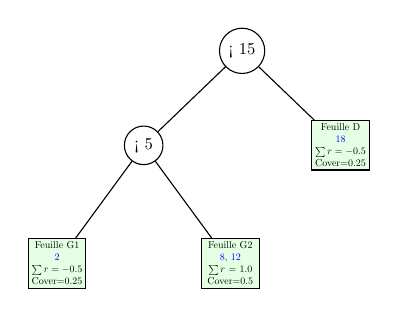
\begin{tikzpicture}[
                    level 1/.style={sibling distance=2.5cm, level distance=1.2cm},
                    level 2/.style={sibling distance=2.2cm, level distance=1.5cm},
                    every node/.style={circle, draw, align=center, scale=0.6},
                    leaf/.style={rectangle, draw, fill=green!10, text width=1.8cm, scale=0.6}
                ]
                \node {< 15}
                    child {node {< 5}
                        child {node[leaf] {Feuille G1 \\ \textcolor{blue}{2} \\ $\sum r=-0.5$ \\ Cover=0.25}}
                        child {node[leaf] {Feuille G2 \\ \textcolor{blue}{8, 12} \\ $\sum r=1.0$ \\ Cover=0.5}}
                    }
                    child {node[leaf] {Feuille D \\ \textcolor{blue}{18} \\ $\sum r=-0.5$ \\ Cover=0.25}};
                \end{tikzpicture}
            \end{block}
        \end{column}
        
        \begin{column}{0.55\textwidth}
            \begin{block}{Valeur de Sortie (Output Value)}
                \scriptsize
                Une fois l'arbre construit, on calcule sa valeur de sortie pour faire des prédictions.
                
                \vspace{0.1cm}
                La formule est la même que le Similarity Score, \textbf{sans le carré au numérateur} :
                $$ \text{Output} = \frac{\sum \text{Résidus}}{\sum \text{Cover} + \lambda} $$
                
                \vspace{0.1cm}
                \textbf{Feuille G1} (Dosage 2) :
                $$ O_{G1} = \frac{-0.5}{0.25} = \textbf{-2.0} $$
                
                \textbf{Feuille G2} (Dosages 8, 12) :
                $$ O_{G2} = \frac{1.0}{0.5} = \textbf{2.0} $$
                
                \textbf{Feuille D} (Dosage 18) :
                $$ O_{D} = \frac{-0.5}{0.25} = \textbf{-2.0} $$
            \end{block}
        \end{column}
    \end{columns}
\end{frame}

% Frame 8 : Mise a jour des Log-Odds
\begin{frame}{XGBoost (Classification) : Mise à jour des Log-Odds}
    \begin{block}{1. Log-Odds de l'étape 1 ($\eta = 0.3$)}
        \small
        On met à jour les Log-Odds initiaux (qui valaient $0$) avec les sorties de l'arbre :
        $$ \text{LO}_1 = \text{LO}_0 + \eta \times \text{Output} $$
        
        \vspace{0.2cm}
        \begin{itemize}
            \item \textbf{Feuilles G1 et D} (Points 2, 18) : \\ 
            $\text{LO}_1 = 0 + 0.3 \times (-2.0) = \textbf{-0.6}$
            
            \vspace{0.2cm}
            \item \textbf{Feuille G2} (Points 8, 12) : \\ 
            $\text{LO}_1 = 0 + 0.3 \times (2.0) = \textbf{0.6}$
        \end{itemize}
    \end{block}
    
    \begin{block}{Pourquoi additionner en Log-Odds ?}
        \small
        L'addition directe de probabilités pourrait nous faire sortir de l'intervalle $[0, 1]$. 
        L'addition dans l'espace Log-Odds (infini) garantit qu'après passage dans la fonction logistique, la probabilité restera \textbf{toujours} cohérente.
    \end{block}
\end{frame}

% Frame 9 : Conversion et Resultat Visuel
\begin{frame}{XGBoost (Classification) : Retour aux Probabilités}
    \begin{columns}[T]
        \begin{column}{0.45\textwidth}
            \begin{block}{Conversion ($p_1$)}
                \scriptsize
                On utilise la \textbf{Fonction Logistique} :
                $$ p_1 = \frac{e^{\text{LO}_1}}{1 + e^{\text{LO}_1}} $$
                
                \begin{itemize}
                    \setlength\itemsep{0.2cm}
                    \item \textbf{F. G1/D} ($\text{LO}=-0.6$) : \\ $p_1 \approx \textbf{0.35}$
                    \item \textbf{F. G2} ($\text{LO}=+0.6$) : \\ $p_1 \approx \textbf{0.65}$
                \end{itemize}
            \end{block}
            
            \vspace{0.2cm}
            \scriptsize
            Les probabilités ne sont plus bloquées à 0.5 ! Le modèle commence à se mouiller.
        \end{column}
        
        \begin{column}{0.55\textwidth}
            \centering
            \textbf{Mise à jour graphique}
            
            \vspace{0.2cm}
            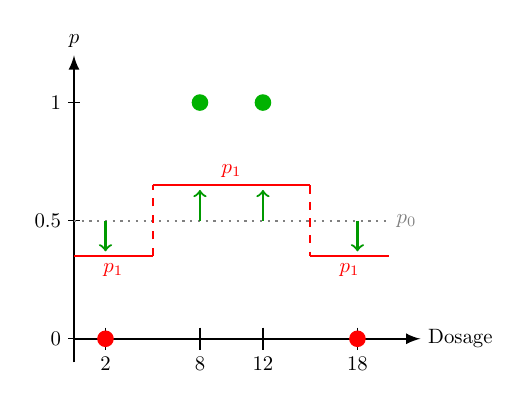
\begin{tikzpicture}[x=0.20cm, y=3cm, every node/.style={scale=0.75}]
                \draw[->, thick, -latex] (0,-0.1) -- (0,1.2) node[above] {$p$};
                \draw[->, thick, -latex] (0,0) -- (22,0) node[right] {Dosage};
                
                \foreach \y in {0, 0.5, 1} { \draw (2pt,\y) -- (-2pt,\y) node[left] {\y}; }
                \foreach \x in {2, 8, 12, 18} { \draw (\x, 4pt) -- (\x, -4pt) node[below] {\x}; }
                
                \draw[thick, gray, dotted] (0, 0.5) -- (20, 0.5) node[right] {$p_0$};
                
                % f1(x) nouveau
                \draw[thick, red] (0, 0.35) -- (5, 0.35) node[midway, below] {$p_1$};
                \draw[thick, red, dashed] (5, 0.35) -- (5, 0.65);
                \draw[thick, red] (5, 0.65) -- (15, 0.65) node[midway, above] {$p_1$};
                \draw[thick, red, dashed] (15, 0.65) -- (15, 0.35);
                \draw[thick, red] (15, 0.35) -- (20, 0.35) node[midway, below] {$p_1$};
                
                % Points
                \fill[red] (2,0) circle (3pt);
                \fill[green!70!black] (8,1) circle (3pt);
                \fill[green!70!black] (12,1) circle (3pt);
                \fill[red] (18,0) circle (3pt);
                
                % Fleches de deplacement
                \draw[->, green!60!black, thick] (8, 0.5) -- (8, 0.63);
                \draw[->, green!60!black, thick] (12, 0.5) -- (12, 0.63);
                \draw[->, green!60!black, thick] (18, 0.5) -- (18, 0.37);
                \draw[->, green!60!black, thick] (2, 0.5) -- (2, 0.37);
            \end{tikzpicture}
        \end{column}
    \end{columns}
\end{frame}

% Frame 10 : Nouveaux Résidus et Itérations
\begin{frame}{XGBoost (Classification) : Itérations Suivantes}
    \vspace{-0.2cm}
    \begin{block}{Calcul des nouveaux résidus ($r_1$)}
        \scriptsize Répétition du processus : $r_1 = y_i - p_1$. L'erreur a globalement diminué !
        
        \vspace{0.1cm}
        \centering
        \begin{tabular}{|c|c|c|c|c|}
            \hline
            \textbf{Dosage} & $y_i$ & \textbf{Ancien } $p_0$ ($r_0$) & \textbf{Nouveau } $p_1$ & \textbf{Nouveau Résidu } $r_1$ \\
            \hline
            2 (R) & 0 & 0.5 (-0.5) & \textbf{0.35} & $0 - 0.35 = \textbf{-0.35}$ \\
            8 (V) & 1 & 0.5 (+0.5) & \textbf{0.65} & $1 - 0.65 = \textbf{+0.35}$ \\
            12 (V) & 1 & 0.5 (+0.5) & \textbf{0.65} & $1 - 0.65 = \textbf{+0.35}$ \\
            18 (R) & 0 & 0.5 (-0.5) & \textbf{0.35} & $0 - 0.35 = \textbf{-0.35}$ \\
            \hline
        \end{tabular}
    \end{block}

    \begin{columns}[T]
        \begin{column}{0.48\textwidth}
            \begin{block}{Construction de l'Arbre 2}
                \scriptsize
                \begin{itemize}
                    \item On construit maintenant un deuxième arbre.
                    \item Son objectif est de prédire ces \textbf{nouveaux résidus} $r_1$ ($\pm 0.35$).
                    \item Les "Covers" seront mis à jour avec les nouveaux $p_1$.
                \end{itemize}
            \end{block}
        \end{column}
        
        \begin{column}{0.52\textwidth}
            \begin{block}{Boucle Algorithmique}
                \scriptsize
                Le processus se répète ($p_2, p_3, \dots, p_M$) jusqu'à :
                \begin{itemize}
                    \item Atteindre le nombre max d'arbres (\texttt{n\_estimators}).
                    \item Atteindre l'\textbf{Early Stopping} (les résidus ne diminuent plus).
                \end{itemize}
            \end{block}
        \end{column}
    \end{columns}
\end{frame}
